\documentclass{article}
\usepackage[ruled]{algorithm2e}
\usepackage{amsmath}
\usepackage{amssymb}
\usepackage{graphicx}
\usepackage{hyperref}
\usepackage{import}
\usepackage{microtype} % better typesetting
\usepackage{subfig}

\let\orgautoref\autoref
\providecommand{\Autoref}
        {\def\equationautorefname{Equation}%
         \def\figureautorefname{Figure}%
         \def\subfigureautorefname{Figure}%
         \def\Itemautorefname{Item}%
         \def\tableautorefname{Table}%
         \def\sectionautorefname{Section}%
         \def\subsectionautorefname{Section}%
         \def\subsubsectionautorefname{Section}%
         \def\chapterautorefname{Section}%
         \def\partautorefname{Part}%
         \orgautoref}

\newcommand{\proc}[1]{\textnormal{\scshape#1}}

\DeclareMathOperator*{\argmin}{argmax}
\DeclareMathOperator*{\argmax}{argmax}
\DeclareMathOperator{\LoG}{\proc{LaplacianOfGaussian}}
\DeclareMathOperator{\Window}{Window}
\newcommand{\floor}[1]{\lfloor #1 \rfloor}

\title{Parallel Stereo Vision}
\author{Michael Koval}
\date{January 1, 2012}

\begin{document}
\maketitle

\section{Introduction}
\label{sec:intro}
Stereo vision is the process of extracting depth information from a
\textit{stereo pair}, or two simultaneous images of a scene that are captured
from different position. Humans unconsciously use stereo vision to perceive
depth, but mimicking this success with a digital cameras and a computer is
quite challenging and---as with many computer vision problems---all of the
known algorithms are computationally intensive. At its heart, the stereo vision
problem requires matching each pixel in the left image of a stereo pair to the
corresponding pixel in the right image of the same pair. The distance between
these two pixels is known as \textit{disparity} and is inversely proportional
to the distance from the imaged point to the camera.

Matching algorithms that solve this problem are special optimization algorithms
that find the optimal pairing of pixels between the left and right images of a
stereo pair for some definition of pairwise similarity. One of the most common
matching algorithms, known as a \textit{block matching} algorithm, define
similarity as a function of only a small rectangular window of pixels
surrounding the candidate pair of pixels. This paper considers the \textit{sum
of absolute difference block matching} (SAD-BM) algorithm proposed by
Konolige~\cite{konolige97} which defines similarity as the sum of element-wise
differences in intensity between blocks because of its relative simplicity,
ability to run in real-time, and the availability of a open-source
implementation to use as a benchmark.

In \Autoref{sec:serial} the basic SAD-BM algorithm and a serial implementation
will be described in detail. Next, the algorithm will be parallelized on the
CPU using OpenMP (\Autoref{sec:parallel-omp}) and on the GPU using NVIDIA'S
CUDA (\Autoref{sec:parallel-cuda}). The performance characteristics of each of
these algorithms is evaluated in \Autoref{sec:perf} and compared against two
highly optimized open source implementations of the same algorithm. Finally, in
\Autoref{sec:future}, several potential performance improvements will be
enumerated.

\section{Serial Algorithm}
\label{sec:serial}
For each pixel in the left image, $p_l$, a stereo matching algorithm attempts
to find $p_r$, the corresponding pixel in the right image such as that $p_l$
and $p_r$ are ``most similar''. In the case of SAD-BM and other block matching
algorithms, the similarity between $p_l$ and $p_r$ is assumed to be the
similarity between the pixels inside the $n \times n$ window centered at $p_l$
and $p_r$. In the case of the Konolige's algorithm ~\ref{konolige97}, the
similarity of two windows is defined as the \textit{sum of absolute
differences} (SAD) or L1-norm of the difference of the two windows, i.e.
\begin{align*}
    p_r = \argmax_p \left|\left|\Window_{m \times n}(I_{left}, p_l)
          - \Window_{m \times n}(I_{right}, p_r)\right|\right|_1
\end{align*}
where $\Window_{m \times n}(I, p)$ is the $m \times n$ rectangle of pixels
centered at point $p$ in image $I$.

Implemented na\"{i}vely, this would be quite inefficient because the algorithm
must exhaustively check every pair of pixels in the left and right images. On a
stereo pair of dimensions $w \times h$, this would require $\Theta(w^2 h^2)$
window comparisons. Using \textit{epipolar geometry}, the geometry of stereo
vision, it is possible to reduce the size of research space by eliminating
corresponding pairs of points that are geometrically impossible\footnote{Any
pair of points that violate the epipolar constraint need not be considered.}.
This theoretical result can be applied to a calibrated camera to
\textit{rectify} the stereo pair and force corresponding points to appear in
the same row in both images\footnote{In terms of epipolar geometric,
rectification is a transformation that forces the epipolar lines to be
row-aligned.} Using a rectified stereo pair, the number of comparisons is
reduced to $\Theta(w h d)$ where $D$ is the maximum possible disparity. As
$D \le w$, this is at least a linear speedup over the na\"{i}ve algorithm.

\begin{figure}
    \centering
    \subfloat[Input Image]{
        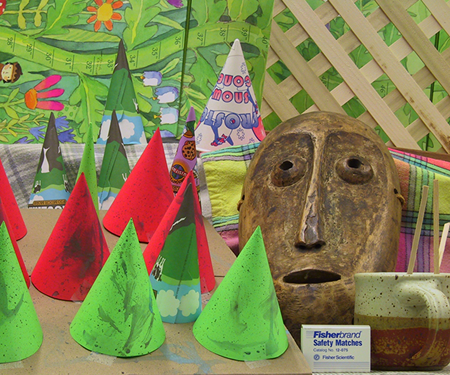
\includegraphics[width=0.33\textwidth]{figures/raw}
    }
    \subfloat[LoG Transformation]{
        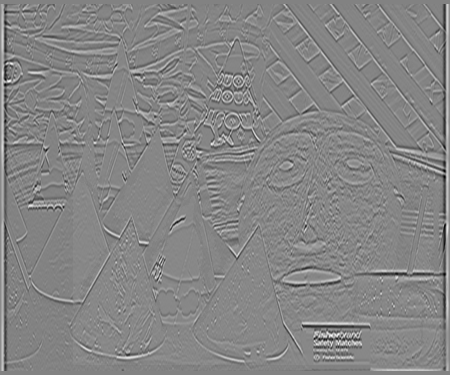
\includegraphics[width=0.33\textwidth]{figures/log}
    }
    \subfloat[Disparity Map]{
        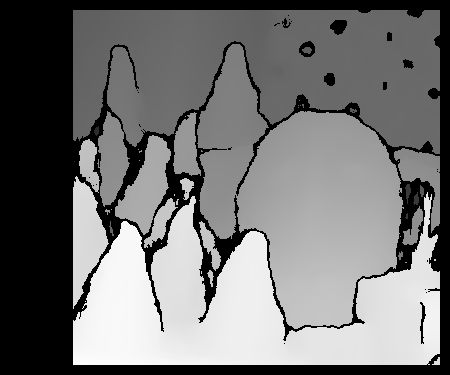
\includegraphics[width=0.33\textwidth]{figures/disparity}
    }
    \caption{
        % TODO
    }
    \label{fig:images}
\end{figure}

This algorithm minimizes the number of pairwise pixel comparisons, but says
nothing of the efficiency of $n \times n$ block comparison. Comparing a pair of
these blocks requires $\Theta(n^2)$ operations and, if all pairs are
independent, the total time complexity is $\Theta(w h D n^2)$. This can be
decreased by using additional memory and calculating a separate vertical
integral images of the SAD error for every possible disparity. Formally, eaach
vertical \textit{integral image} of error is
\begin{align*}
    I_{integral}^{(d)}[x, y] = \sum_{y' = 0}^y I^{(d)}[x, y],
\end{align*}
where $I^{(d)}$ is an image that contains the horizontal SAD error for each
pixel at disparity $d$. Computing each of the $d$ vertical integral images has
time complexity $\Theta(w h n)$. Given the integral images, the error in an $n
\times n$ window can be calculated in constant time. Therefore, the total time
complexity of the algorithm is $\Theta(w h d n)$ with $\Omega(w h)$ memory
overhead\footnote{This assumes that each disparity is calculated in series so
only one integral image is in memory at a given time.}

\begin{algorithm}
    \KwIn {$I_{left}, I_{right} \in \mathbb{R}^{w \times h}$: rectified stereo pair}
    \KwIn {$n \in \mathbb{Z}$: width and height of SAD windows}
    \KwIn {$D \in \mathbb{N}_w$: maximum disparity}
    \KwOut {$I_{disp} \in \mathbb{N}_d^{w \times h}$: disparity map}
    $I_{left}^{(log)} \gets \LoG(I_{left})$   \;
    $I_{right}^{(log)} \gets \LoG(I_{right})$ \;
    %\STATE \COMMENT {compute vertical integral images of error}
    \For {$d = 1 \to D$} {
        \ForEach {$(x_0, y_0) \in \mathbb{N}_w \times \mathbb{N}_h$} {
            $E_y^{(d)} \gets \sum_{\Delta x = -n/2}^{n/2} \left(
                          I_{left}^{(log)}[x_0 - \Delta x, y_0]
                          - I_{right}^{(log)}[x_0 - \Delta x - d, y_0] \right)$ \;
            $I_{sad}^{(d)}[x, y] \gets E_y + I_{sad}^{(d)}[x, y - 1]$ \;
        }
    }
    %\STATE \COMMENT {choose the disparity for each pixel that minimizes error}
    \ForEach {$(x_0, y_0) \in \mathbb{N}_w \times \mathbb{N}_h$} {
        $I_{disp}[x, y] \gets \argmin_{d \le D} I_{sad}^{(d)}[x, y + n/2] - I_{sad}^{(d)}[x, y - n/2]$ \;
    }
    \Return {$I_{disp}$}
    \caption{
        TODO
    }
    \label{alg:serial}
\end{algorithm}

\section{Parallelization}
\label{sec:parallel}

\subsection{OpenMP}
\label{sec:parallel-omp}
This is a multi-step algorithm, where each step depends entirely on the output
of the previous step (e.g. error processing cannot begin until after the LoG
transformation is finished). This means that parallelizing each stage in the
algorithm is equivalent to parallelizing the entire algorithm.

First, consider the two-dimensional convolution required in the LoG
transformation. Assuming all images are stored in row-major order, this can be
done by assigning each thread a row, column, or single pixel. Given a
sufficient number of cores, assigning each pixel a thread would be ideal.
Unfortunately, modern CPUs have a small number of cores and the overhead of
assigning one thread to each pixel would negate any performance gain from doing
so. Instead, the rows of the image will be partitioned into groups of
contiguous rows by OpenMP. This allows the number of threads to be tuned to
match the CPU's number of cores and guarantees that each thread will
sequentially accesses memory.

Once the LoG transformation is complete, the next step is to compute integral
images of the SAD error. Unlike with the LoG, this cannot be done by
partitioning the data into rows: each row depends on all previous rows. One
potential solution is to partition the data into columns. Unfortunately, this
grossly inefficient because this splits sequential memory accesses across
threads. This can be improved by spitting the calculation of integral images
into two steps: first partition the image into rows to compute the horizontal
component of the integral image, then sum along columns in parallel. This has
the same complexity of computing the integral in one pass, but reduces the
number of non-sequential memory accesses.

Once the integral images have been computed, the disparity of each pixel can be
independently computed and stored in the disparity map. For the same reason as
with the LoG transform, the integral images were partitioned into rows for this
calculation. Since each of these operations can be parallelized with no thread
synchronization the resulting algorithm should linearly speedup with the number
of threads until the number of threads exceeds the width or the height of the
images. In practice, there will also be a small amount of constant overhead 
while waiting for the threads to synchronize between steps of the algorithm.

\subsection{NVidia CUDA}
\label{sec:parallel-cuda}
Unlike OpenMP, in which threads are high overhead, NVidia's CUDA architecture
allows for zero-overhead threads and SIMD instructions. However, this comes at
a cost: memory transfers between the CPU and GPU are extremely costly and must
be minimized to achieve respectable performance. Specifically, this means that
the stereo pair is transferred to the GPU as a single unit, all processing
should occur on the GPU, then the resulting disparity map is copied back to the
CPU as a single operation.

Once the transfer is complete, the LoG is easy to compute: each pixel in the
image is assigned a thread and all of the corresponding output pixels are
computed in parallel. While this would be very inefficient on the CPU because
of the overhead of traditional threads, this is ideal for the massively
parallel architecture and zero-overhead threads available on the GPU. Even
with assigning one pixel per thread, it still must be decided how to partition
the threads into blocks. For optimal performance the number of threads per block
must be a multiple of the warp size, $W$, however, this says nothing about how the
threads should be partitioned into blocks. To minimize the number of memory
accesses---the slowest operation---per block, this was done by partitioning the
image into blocks of size $\floor{\sqrt{W}} \times \floor{\sqrt{W}}$.

Once the LoG of the input images have been calculated, the next step is to
compute the integral images. This can be done using the same technique as
described in \Autoref{sec:omp}; by computing the horizontal SAD, then summing
along columns in the resulting image. Computing the horizontal SAD can be done
using square blocks of size $\floor{\sqrt{W}} \times \floor{\sqrt{W}}$ and the
same partitioning scheme as described above. Summing the image vertically
cannot use this partitioning because rows are inter-dependent. Since columns
are independent, each column is assigned a thread and is grouped into a block
of size $1 \times W$. This is non-ideal, but is the only way of eliminating
inter-thread communication.

Finally, the integral images are reduced to a disparity map using the same
algorithm as described in \Autoref{sec:omp}. Just as with the LoG
transformation, each pixel is assigned a thread and is assigned to a
$\floor{\sqrt{W}} \times \floor{\sqrt{W}}$ block. Once the disparity image has
been computed it either remains on the GPU for further CUDA-accelerated
operations or, more likely, is copied back to the host for manipulation on the
CPU.

\section{Performance Analysis}
\label{sec:perf}
The serial algorithm, OpenMP parallelized algorithm, and the CUDA parallelized
algorithm were each implemented in C++ using OpenCV data structures. In
addition, OpenCV was built with CUDA support so the open-source CPU and GPU
implementations of the algorithms could be evaluated. Each of these algorithms
was evaluated on the 2003 Middlebury stereo dataset and the results were
compared with ground truth to verify that each implementation was producing
valid output. Since the runtime of the algorithm is deterministic in the size
and bitdepth of the image, the \textit{cones} was arbitrary selected. The
parameters of the SAD-BM algorithm were set to $D = 64$ and $n = 21$, values
that are typical when the algorithm is used in real-time. The results of this
performance evaluation are shown in \Autoref{fig:perf}

\begin{figure}
    \centering
    \subimport{figures/}{threads}
    \caption{
        Performance of the OpenMP algorithm evaluated on a machine with a 24
        cores, 800 MHz processor and a NVidia Teslda C2070 GPGPU. In
        \ref{fig:perf-omp} the number of threads is varied. Note the
        diminishing returns from Amdahl's law and the peak in performance at 24
        threads.
    }
    \label{fig:perf-omp}
\end{figure}

As \Autoref{fig:perf-omp} shows, parallelizing SAD-BM with OpenMP performs as
was predicted in \Autoref{sec:parallel-omp}; performance increases subject to
until the number of threads exceeds the number of CPU cores, at which point
performance decreases due to the overhead of additional threads. While the
parallel performance increase is impressive, it still suffers from diminishing
returns. This is consistent with Amdahl's law, which says that the maximum
speedup of an algorithm is limited by the sections of the algorithm that cannot
be serialized. In this case, much of that overhead is caused by splitting the
algorithm into several smaller stages and could be improved by pipelining the
calculating so the stages can run in parallel (see \Autoref{sec:future} for
details).

\begin{figure}
    \centering
    \subimport{figures/}{comparison}
    \caption{
        Comparison between algorithms described in this report and the open
        source implementations in OpenCV. Note that the GPU accelerated
        algorithms outperform the CPU algorithms and the OpenCV implementations
        outperform the custom implementations in all cases.
    }
    \label{fig:perf-comp}
\end{figure}

Overall, the OpenMP parallelization gave a large performance increase without
any additional complexity: parallelizing the serial algorithm with OpenMP
simply required adding three preprocessor directives! Despite this boost in
performance, this algorithm runs 6.15 times slower than the OpenCV
implementation (\Autoref{fig:perf-comp}). The impressive performance of OpenCV
is attributed to three factors: (1) utilizing architecture-specific
instructions, (2) managing threads at a lower level, and (3) hand optimization.
In particular, the OpenCV implementation of SAD-BM makes heavy use of Streaming
SIMD Extensions (SSE2) to perform multiple arithmetic operations in each clock
cycle. Combined with manually-controlled thread synchronization using Intel's
Thread Building Blocks (TBB) and manual loop unrolling, this easily accounts
for the performance difference.

Also as expected, the CUDA-accelerated SAD-BM algorithm is 2.71 times faster
than the OpenMP parallelized CPU algorithm. This is surprisingly poor
performance because the SAD-BM algorithm---like many computer vision
algorithms---is particularly well-suited for massive parallelism. This speedup
is lower than, but comparable to, OpenCV's the 7.37 times performance
difference between the CPU and GPU algorithms. This performance difference is
harder to attribute, but is most likely from intelligent use of CUDA streams
and manually unrolling loops. Using streams allow for more operations to be
executed in parallel, which is exceptionally important when working on powerful
GPGPUs like the NVidia Tesla in the machine used for evaluation.

\section{Conclusion}
\label{sec:conc}
Overall, the results (\Autoref{fig:perf-comp}) show that parallelizing the
SAD-BM algorithm can significantly improve performance. Using CPU threads on a
multi-core processor yields a considerable speedup without requiring any
expensive hardware and very minimal changes to the serial algorithm. Indeed,
running the OpenMP-parallelized algorithm with one thread is exactly equivalent
to running the serial algorithm. Note, however, that this implementation is
heavily affected by the number of CPU cores. While the performance is excellent
on a 24-core machine, it will likely be disappointing on more common dual or
quad core machines. This is in contrast to the CUDA implementation, which
necessitated reimplementing the entire algorithm from scratch.

If a high end GPGPU is available and performance is critical, then GPU
acceleration cannot be matched. Both of the CUDA-accelerated implementations
outperformed their corresponding multi-threaded CPU implementations. This is
especially important when the CPU is under heavy load because offloading
computations to the GPU frees up additional CPU time for other tasks. One
example of this is on a robot that much simultaneously perceive obstacles with
stereo vision and plan paths around the observed obstacles. Even if the CPU was
fast enough to run the SAD-BM algorithm in real-time, doing the calculations on
the GPU would allow more CPU time to be spent on path planning.

\section{Future Work}
\label{sec:future}
From the comparison with OpenCV, there are obviously improvements that can be
made in this implementation. On the CPU this would involve: (1) using SSE2 to
perform multiple arithmetic calculations per clock cycle, (2) manually unroll
tight loops to reduce overhead, and (3) switching to a lower-level threading
library to reduce the amount of synchronization. On more modern processors, the
SSE4.1 SIMD instructions for SAD calculation could be used to even greater
effect by allowing an $8 \times 8$ SAD window to calculated in seven clock
cycles. These instructions are not used in OpenCV, so this is a potential
method of surpassing OpenCV's performance.

Optimizations are less obvious on the GPU. Most importantly, the code should be
modified to use CUDA streams to pipeline operations and minimize the number of
synchronizing points. Another major optimization would be to replace some
custom code, such as the LoG convolution, with NVidia Performance Primitives
(NPP) that are already highly optimized. At a lower level, performance could be
improved by padding images to be a multiple of the block size and manually
unrolling loops to minimize bounds checking in the kernels. Together, these
improvements would close the gap between this implementation of SAD-BM and the
highly optimized open source implementation in OpenCV.

\bibliography{report}{}
\bibliographystyle{plain}

\end{document}
